\documentclass[11pt]{article}

\usepackage{url}
\usepackage[utf8x]{inputenc}
\usepackage{minted}
\usemintedstyle{emacs}
\usepackage{cite}
\usepackage[pdftex]{graphicx}
\usepackage{amsmath}
\usepackage{subcaption}
\usepackage[table,x11names]{xcolor}

\usepackage[titletoc,title]{appendix}

\usepackage[margin=1in]{geometry}
\usepackage[doublespacing]{setspace}
\usepackage{lscape}

\hyphenation{}


\begin{document}

\title{Topic mining for short-text documents on a micro-blogging site with Doc2Vec and clustering and its application to influence mining}


% author names and affiliations
\author{Thuong-Hai Pham and Carlos F. Diez Sánchez\\
Faculty of Information and Communication Technology\\
University of Malta\\
Msida MSD 2080, Malta}

% make the title area
\maketitle

% As a general rule, do not put math, special symbols or citations
% in the abstract
\begin{abstract}
In the era of data explosion, especially digital text generated by World Wide Web users, there is an increasing demand for techniques that automatically organise large collections of texts for further analysis and other processing tasks. One of this set of techniques is called "topic model". These techniques discover underlying topics from a given corpus with or without human intervention. This report examines the traditional Latent Dirichlet Allocation (LDA) and a proposed method that combines Doc2Vec and a clustering technique on the problem of topic mining. As for the practical evaluation, Twitter\footnote{https://twitter.com/} was chosen to run the experiments, with three different approaches: standard LDA, author-topic model and our own proposed approach. We also cover the background behind each method and report the difficulties when attempting to make use of our topic mining results for topic-sensitive influencers mining task with real life data.

\end{abstract}

% no keywords

\section{Introduction}

Applying topic model for micro-blogging sites is a very important task to enhance our understanding of the social networks. One very successful technique and also being considered as state-of-the-art in unsupervised topic model is Latent Dirichlet Allocation (LDA)\cite{Blei2003}. Some applications were proposed by Zhao et al. (2011) \cite{zhao2011comparing} with a study comparing Twitter and traditional media with LDA, or finding topic-sensitive influencers on Twitter by Weng et al. (2010) \cite{Weng2010}.

It is important to note that applying LDA directly on micro-blogging sites is considered to be not a trivial task, but rather a challenging problem. This occurs due to the nature of micro-blogging sites, which is the limited length of each posting unit (e.g. tweets on Twitter have maximum 140 characters each). In order to solve this problem, our proposed solution with LDA has to make more assumptions (i.e. single-topic tweets) \cite{zhao2011comparing} about the data itself other than the bag-of-words (BOW) assumption from original LDA.

Therefore, we consider examining a clustering method, such as K-means, to discover the underlying topic. The feature learning is done by Doc2Vec by Le \& Mikolov\cite{le2014distributed}, which is an adaptation of Word2vec\cite{mikolov2013distributed}.

As for the rest of this report, in Section \ref{background}, we discuss the mathematical background behind the BOW assumption for topic model: the infinite exchangeability and De Finetti theorem. Thereafter, we revise LDA as a generative probabilistic model and its latent variables in Section \ref{lda}. However, LDA does not work well when applying it directly to short-text documents as tweets. We then consider two variants of LDA to solve this problem, which are author-topic model (\ref{author_topic}) and Twitter-LDA (\ref{twitter_lda}). To end with the background and related works, the three groups of methods to evaluate topic models are also mentioned in Section \ref{evaluation}. To end with, we figure out the disadvantages of these methods and present our proposal in Section \ref{proposal}.

% TODO: add more


\section{Background} \label{background}


\subsection{Mathematical background} \label{math}

\subsubsection{Exchangeability}

We say that $(x_1,x_2...)$ is an infinitely exchangeable sequence of random variables if, for any $n$, the joint probability $p(x_1,x_2,...,x_n)$ is invariant to the permutation of the indices. That is, for any permutation $\pi$,
\[p(x_1,...,x_n) = p(x_\pi(1),...,x_\pi(n))\]
It is important to emphasise that independent and identically distributed random variables are always infinitely exchangeable. However, infinite exchangeability is a much broader concept than being independent or identically distributed. For example, let $(x_1,x_2,\dots)$ be independent and identically distributed, and let $x_0$ be a non-trivial random variable independent of the rest. Then $(x_0+x_1,x_0+x_2,\dots)$ is infinitely exchangeable but not independent and identically distributed.

\subsubsection{De Finetti theorem, 1935}
A sequence of random variables $(x_1,x_2,...)$ is infinitely exchangeable iff, for all $n$,
\[p(x_1,x_2,...,x_n)=\int\prod_{i=1}^{n}p(x_i|\theta)P(d\theta)\]
for some measure $P$ on $\theta$.
If one assumes the data is infinitely exchangeable, then there must exist an underlying parameter and prior.

\subsection{Latent Dirichlet Allocation} \label{lda}

LDA is a generative probabilistic model of a corpus. The basic idea is that documents are represented as random mixtures over latent topics, where a topic is characterised by a distribution over words. To implement this idea, LDA assumes each document is a bag of words (BOW assumption). Hence, it applies infinite exchangeability on the documents and inherits the De Finetti theorem to expect a latent parameter and prior underlying in the corpus. These latent variables are illustrated in the Figure \ref{fig:lda_model} below.


\begin{figure}[ht]
	\centering
	
\includegraphics[scale=0.3]{lda_model}
	\caption{LDA graphical model}
	\label{fig:lda_model}
\end{figure}

In Figure \ref{fig:lda_model}:
\begin{itemize}
	\item $\alpha$ is Dirichlet distribution parameter, controls the shape and sparsity of $\theta$
	\item $\theta$ are per-document topic proportions.\\
	$\theta$ is a K-dimensional Dirichlet random variable, it takes values in the (k-1)-simplex, and has the following probability density on this simplex:
	\[p(\theta|\alpha)=\frac{\Gamma(\sum_{i=1}^{K}\alpha_i)}{\prod_{i=1}^{K}\Gamma(\alpha_i)}\theta_1^{\alpha_1-1}\dots\theta_K^{\alpha_K-1}\]
	The Dirichlet is conjugate to the multinomial. Given a multinomial observation, the posterior distribution of $\theta$ is a Dirichlet.
	\item $Z_{d,n}$ is per-word topic assignment, in which $D$ and $N$ are the number of documents and number of words in a specific document, respectively.
	\item $W_{d,n}$ is the observed word.
	\item $\beta$ are the topics, which is $V$ dimensional Dirichlet.
	\item $\eta$ is the topic hyper parameter.
\end{itemize}

The blue-shaded node denotes the observed variable, the others are hidden or latent variables. Plates denote the replicated structures.

From a collection of documents, LDA infers: per-word topic assignment $Z_{d,n}$, per-document topic proportions $\theta_d$ and per-corpus topic distributions $\beta_k$.

\subsubsection{Generative process}

As mentioned above, LDA is a generative probabilistic model, whose generative process is performed as described below:
\begin{enumerate}
	\item Draw $\theta_d \sim Dir(\alpha)$
	\item Draw $\beta_k \sim Dir(\eta)$
	\item For each of the N words in document d $W_{d,n}$:
	\begin{enumerate}
		\item Draw a topic $Z_{d,n} \sim Multinomial(\theta_d)$
		\item Draw a word $W_{d,n}$ from $p(W_{d,n}|Z_{d,n},\beta)$, a multinomial probability conditioned on the topic $Z_{d,n}$
	\end{enumerate}
\end{enumerate}

\subsubsection{Model inference}
However, the problem is to acquire underlying latent topics, so we have to reverse the generative process by solving an inferential problem. The main goal of this inferential problem is to compute the posterior distribution of the latent variables in Figure \ref{fig:lda_model}:
\[p(\theta,Z|W,\alpha,\beta)=\frac{p(\theta,Z,W|\alpha,\beta)}{p(W|\alpha,\beta)}\]

In practice, is not possible to compute the function $p(\theta,Z|W,\alpha,\beta)$. Due to the conjugacy of the Dirichlet distribution, we can marginalise over latent variables to rewrite the posterior $p(W|\alpha,\beta)$. This posterior is still hard to infer exactly. Nevertheless, there is a wide variety of approximate inference algorithms for LDA:
\begin{itemize}
	\item Mean field variational methods \cite{blei2004variational} (Blei et al., 2001)
	\item Expectation propagation \cite{minka2002expectation} (Minka and Lafferty, 2002)
	\item Collapsed Gibbs sampling \cite{griffiths2004finding} (Griffiths and Steyvers, 2004)
	\item Collapsed variational inference \cite{teh2006collapsed} (Teh et al., 2006)
\end{itemize}

After being approximated, beside LDA, the posterior can be used in many other applications such as collaborative filtering, document similarity and information retrieval...

\subsection{Latent Dirichlet Allocation variants for Twitter} \label{lda_app}

One very basic approach is to apply LDA directly to Twitter by treating each tweet as a single document. However, due to the constraint of 140 characters per tweet, a tweet is too short for LDA to figure out the topic proportions.

\subsubsection{The author-topic model} \label{author_topic}

To overcome this issue, Weng et al. (2010), and Hong \& Davison (2010) \cite{Weng2010,hong2010empirical} proposed the idea of aggregating all tweets of a Twitter's user into a single document, by excluding the topic proportions for each tweet but yet taking into consideration the underlying topics in each user, and obtained better results than the direct LDA.

On one hand, this approach is very efficient on a specific task (e.g. topic-sensitive influencers mining \cite{Weng2010}) because it does not modify the inference process of original LDA. On the other hand, the target of this approach is each user, not the tweets, so it is not applicable for a general problem of topic mining.

\subsubsection{Twitter-LDA} \label{twitter_lda}

On a different perspective, while attempting to compare Twitter and traditional media, Zhao et al. \cite{zhao2011comparing} proposed Twitter-LDA, a modified version of LDA to work with Twitter's short tweets without concatenating all tweets into one.

\begin{figure}[H]
	\centering
	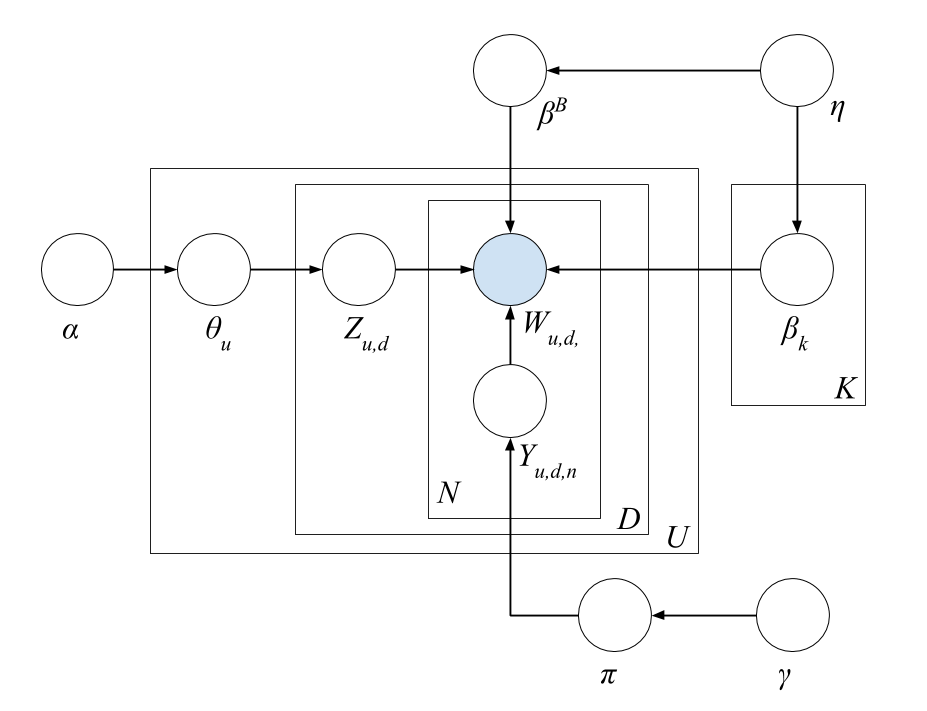
\includegraphics[scale=0.3]{twitter_lda_model}
	\caption{Twitter-LDA graphical model}
	\label{fig:twitter_lda_model}
\end{figure}

In figure \ref{fig:twitter_lda_model}, the author introduced four more variables:
\begin{itemize}
	\item $\beta^B$ denotes the background word distribution
	\item $\pi$ denotes the Bernoulli distribution, which simulates the choice of authors between topic-related words and background words.
	\item $\gamma$ is the parameter of distribution $\pi$.
	\item $Y_{u,d,v}$ denotes the selection of background or topic word.
\end{itemize} 
and a slight modification on $\theta$, where that $\theta_u$ represents the per-user topic proportions, instead of the per-document one, as in the original version. In addition, the D (document) plate is surrounded by a new plate U which stands for each user. It is necessary to mention that Twitter-LDA assumes that each tweet conveys only a single topic. We will clarify our disagreement on this assumption in Section \ref{proposal}.

By defining the model as in figure \ref{fig:twitter_lda_model}, the generative process of Twitter-LDA is performed as followed:
\begin{enumerate}
	\item Draw $\beta^B \sim Dir(\eta)$
	\item Draw $\pi \sim Dir(\gamma)$
	\item Draw $\beta_k \sim Dir(\eta)$
	\item For each user,
	\begin{enumerate}
		\item Draw $Z_{u,d} \sim Multi(\theta_u)$
		\item For each word in document d,
		\begin{enumerate}
			\item Draw $Y_{u,d,n} \sim Multi(\pi)$
			\item Draw \[W_{u,d,n} \sim 
			\begin{cases}
			Multi(\theta^B) & \text{if $Y_{u,d,n} = 0$}\\
			Multi(\theta^{Z_{u,d}}) & \text{if $Y_{u,d,n} = 1$}
			\end{cases}\]
		\end{enumerate}
	\end{enumerate}
\end{enumerate}

\subsection{Evaluation} \label{evaluation}

Wallach et al. \cite{Wallach2009a} summarised a variety of methods to evaluate LDA. As a topic model method, LDA is commonly evaluated with the intrinsic and extrinsic evaluation. 

\subsubsection{Intrinsic evaluation}
One very basic intrinsic evaluation method is to view the problem as document modelling \cite{Blei2003}. The goal of the model is to achieve a high likelihood on a held-out test set, $C'$. In this case, the perplexity measure is used as in normal language modelling problems, where the lower the perplexity is, the better performance the model achieves.
\[perp(C')=exp\left\{-\frac{\sum_{d=1}^{D}{log(p(W_d))}}{\sum_{d=1}^{D}N_d}\right\}\]

In a more advanced way, measurement is also estimated by the probability of unseen held-out documents given some training documents. This probability can be written as
\cite{Wallach2009a}
\[P(C|C')=\int d\theta d\alpha dm P(C|\theta,\alpha m)P(\theta,\alpha m|C').\]
where, $C, C'$ denotes the training document set (corpus) and held-out document set, respectively. Noted that $m$ is the base measure of the Dirichlet distribution, in addition to the concentration parameter $\alpha$.

There is also a variation of this method, document completion, where given the first half of each document, it compares the predictive performance by estimating the probability of the second half. In this point of view, let $c^{(1)}$ be the first half and $c^{(2)}$ be the second half, the goal of our measurement is to compute
\[P(w^{(2)}|w^{(1)},\theta,\alpha m)=\frac{P(w^{(2)}, w^{(1)}|\theta,\alpha m)}{P(w^{(1)}|\theta,\alpha m)}\]

\subsubsection{Extrinsic evaluation}
On the other hand, extrinsic approaches measure LDA performance on some secondary tasks, such as corpus comparison \cite{zhao2011comparing} or topic-sensitive influencers mining \cite{Weng2010}. These approaches are similar to how the performance of language models are measured.

\subsubsection{Human evaluation}

As a part of the corpus comparing works \cite{zhao2011comparing}, Zhao et al. also evaluated the performance between original LDA, author-topic model and their proposed Twitter-LDA. Based on preliminary experiments, the authors set number of topic K to 110 for each model, then mixed 330 topics from the three models. The topics were then scored by two human judges. Each assigned a score on each topic, ranging from 1 (meaningful) to 0 (nonsense).

The result showed that Twitter-LDA gained 25.23\% higher than the author-topic model in terms of average score, and 32.61\% higher than the standard LDA. Hence, Twitter-LDA obviously outperformed the two previous methods and were used for the comparison task.


\section{Proposed method} \label{proposal}

Both methods, author-topic model and Twitter-LDA, have overcome the problem of the tweets' size in the micro-blogging site Twitter, which prevented the direct usage of the original LDA. More than that, it has been showed that Twitter-LDA outperforms the other two in capturing more meaningful topics. Nevertheless, Twitter-LDA has to change the original LDA process and inference approximation algorithm for its implementation. This approach is hard to be re-implemented in the industrial sector by using existing libraries for other problems.

More than that, it is worth to consider the underlying assumption, where one tweet belongs only to one topic, as intended by its Twitter user. However, please note that this topic is not the final topic discovered by our mining methods, but possibly a combination of topics. For example, the topic user intends to tweet about his public insurance. Throughout the whole corpus, our mining process points out two distinct topics: health care and public administration. It is obvious that the user-intended topic reflects the two discovered topics in the perspective of the whole corpus.

Bearing that in mind, we would like to propose a method to compare the original LDA and the author-topic model, by accepting the BOW assumption only.

\subsection{Clustering based on distributed representation of sentences} \label{doc2vec}

\subsubsection{Distributed representation of sentences for feature learning}

Once Word2vec\cite{mikolov2013distributed} had been presented, Le and Mikolov introduced the paragraph (document) vector models. Formally, the objective of a word embedding model is to maximise the log probability

\[\frac{1}{T}\sum_{t=k}^{T-k}\log p(w_t|w_{t-k},\dots,w_{t+k}) \]
given a sequence of training words $w_1,w_2,w_3,\dots,w_T$.

% TODO: more about transition from word2vec to doc2vec

The paragraph vector model uses the same idea to develop the paragraph vector framework. In fact, this is not a single model, but two different approaches: Distributed Memory model (DM) and Distributed Bag of Words (DBOW), a vector without word ordering.

\begin{figure}[ht]
	\centering
	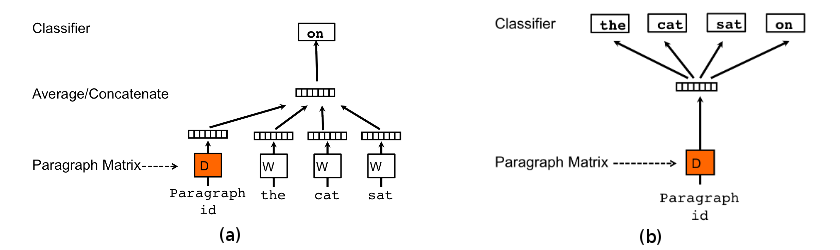
\includegraphics[width=\textwidth]{doc2vec}
	\caption{Framework for learning paragraph vector, (a) Distributed Memory and (b) Distributed Bag of Words.}
	\label{fig:doc2vec}
\end{figure}

In Figure \ref{fig:doc2vec} above,\footnote{https://arxiv.org/pdf/1405.4053v2.pdf} the DM model (a) is actually built from the structure of each word vector (sentence/document), then these vectors are combined (through averaging or concatenation) to learn the sentence/document features. In addition to this, a paragraph matrix keeps track of the whole sentence/document. On the contrary, the DBOW model does not combine any word vectors, yet only a paragraph vector is trained to predict the context.

\subsubsection{Clustering based on the learnt features}
Our proposed method consists of two different parts. First, the "meaning" or, in fact, the features of each document are learnt by the Doc2Vec model, as presented above. Once the features are extracted, the documents are clustered. For the goal of our experiment (described in \ref{evaluation}), we chose K-means to find hard clusters from our documents, Each cluster represents a topic, however, to produce a probabilistic topic proportions as in LDA, we can easily change K-means to C-means to achieve fuzzy or soft clusters.

% TODO: more about parameters used

\section{Experiment} \label{experiment}

The data for this project was acquired from the Archive Team's Twitter Stream Grab (a collection in the JSON format collected from the general Twitter stream) in July 2016.\footnote{https://archive.org/details/archiveteam-twitter-stream-2016-07} Although we could have streamed the data directly from Twitter's Streaming APIs, data preprocessing still plays an essential role to filter out tweets in other languages (Chinese, Japanese, Spanish...), remove stop-words, tokenise words within tweets, remove urls and normalise unconventional language used on social networks (character repetition, emoticons, etc.).

\subsection{Implementation}
The source-code used for the latter evaluation is developed using LDA and Doc2Vec model in Gensim library.\footnote{\url{https://radimrehurek.com/gensim/}}


\subsection{Resources} \label{resources}

Due to the magnitude of our data (48.7GB in compressed format), a sufficiently efficient machine is required to perform data preprocessing and calculation for our experiment. For this reason, we made use of the Compute Engine cloud n1-standard-4.\footnote{operates with 4 virtual CPUs, 15GB RAM, 200GB hard disk drive} In addition, the experiment evaluation process also required to employ two judges (the more, the better) to individually score meaningfulness of our topic mining result.

\subsection{Evaluation}

For the evaluation task, although perplexity is considered to justify the result with less subjectivity, it does not measure how meaningful the topics discovered are. Hence, we make use of the human evaluation strategy\cite{zhao2011comparing} instead. This evaluation process is performed by two distinct judges. Each judge assigns a name for every one of the topics in the output results, with a meaningfulness score from 0 to 10. 
Afterwards, their topic names and scores are exchanged and they score again how much they agree with the other judge's evaluation in a similar scale from 0 to 10. The meaningfulness of each approach is measured by averaging all the agreement scores above, which basically reflects the interpretability of the result.

\section{Topic mining results}
Each experiment divided 606,631 tweets (from the top 1,600 users when they were separated) or 1,600 documents by aggregating tweets from 1,600 users (in case of the author-topic methods) into 20 topics. Afterwards, the two judges scored each one of the topics according to 1) topic assignment, and 2) topic meaningfulness. We then obtained the average for each one of the scores. The visualisation (obtained by applying t-SNE to 2 dimensions) of the four experiments in Figure \ref{fig:res_distribution} shows our intuitive impression that Doc2Vec methods have a better documents-topic distribution, where documents of different topics are spread further from each other. The results in detail will be discussed further in the following section.
% Figure 4 shows a much better grouping of topics when the tweets were separated. 

\begin{figure}[H]
    \centering
    \begin{subfigure}{.49\linewidth}
    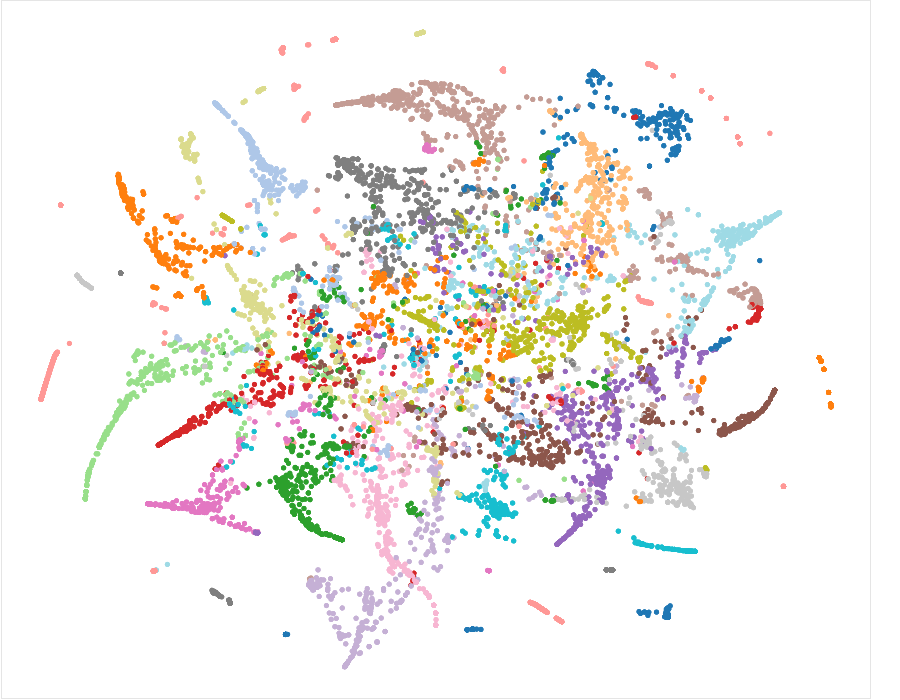
\includegraphics[width=\linewidth]{lda_sep}
    \caption{LDA (tweets separated)}\label{fig:res_lda_sep}
    \end{subfigure}
    \begin{subfigure}{.49\linewidth}
    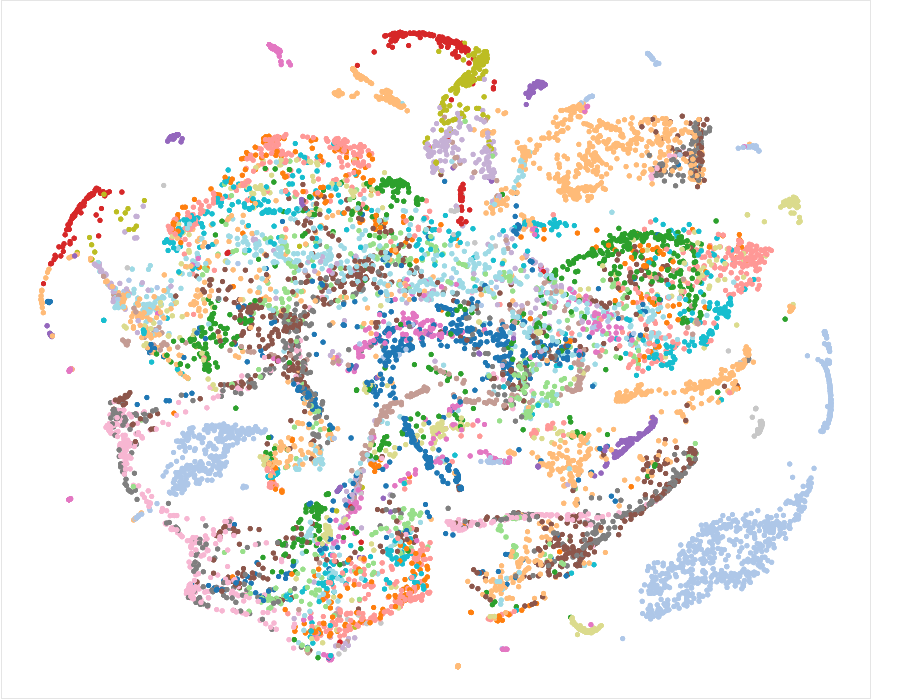
\includegraphics[width=\linewidth]{doc_sep}
    \caption{Doc2Vec (tweets separated)}\label{fig:res_doc_sep}
    \end{subfigure}
    
    \begin{subfigure}{.49\linewidth}
    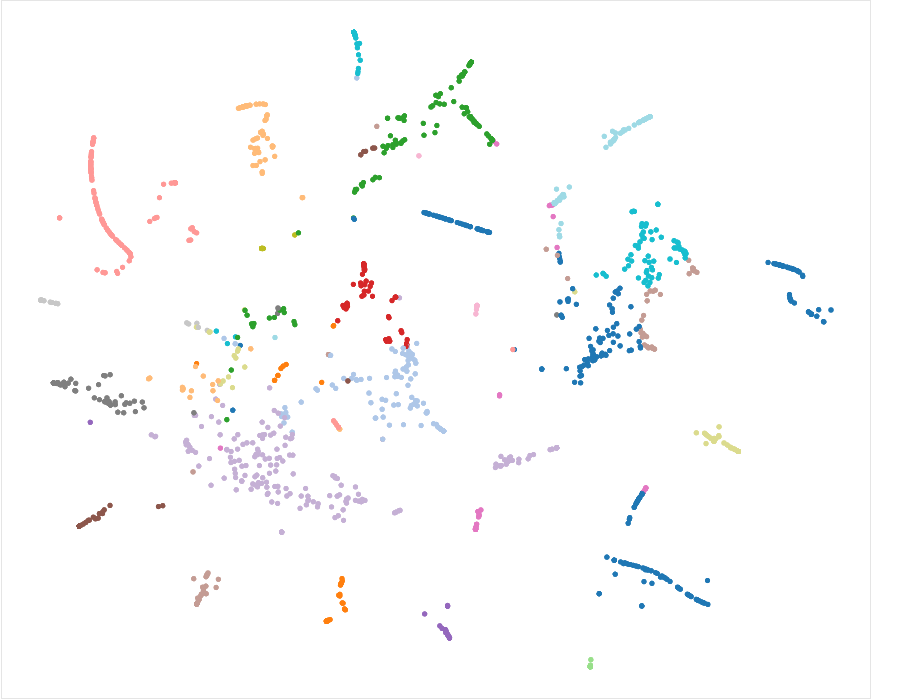
\includegraphics[width=\linewidth]{lda_grp}
    \caption{LDA (author-topic)}\label{fig:res_lda_grp}
    \end{subfigure}
    \begin{subfigure}{.49\linewidth}
    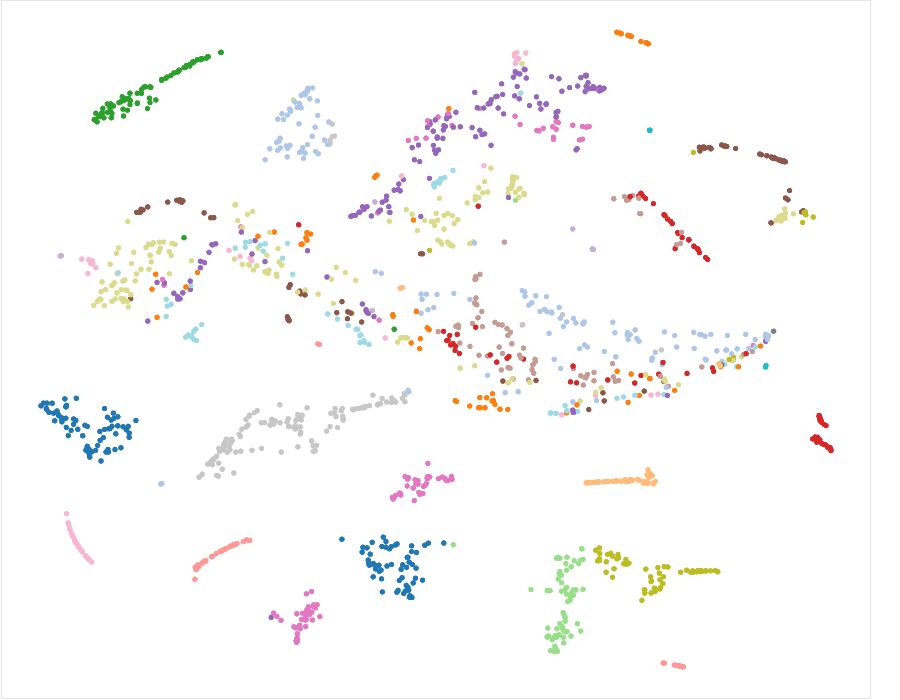
\includegraphics[width=\linewidth]{doc_grp}
    \caption{Doc2Vec (author-topic)}\label{fig:res_doc_grp}
    \end{subfigure}
    
    \caption{Topics and documents (tweets) distributions.}
    \label{fig:res_distribution}
\end{figure}

\begin{table}[H]
	\centering
	\begin{tabular}{| l | p{2.5cm} | p{2.5cm} | p{2.5cm} | p{2.5cm} |}
		\hline
		& \textbf{LDA\newline (tweets separated)} & \textbf{LDA (author-topic)} & \textbf{Doc2Vec (tweets separated)} & \textbf{Doc2Vec (author-topic)}\\
		\hline
		\textbf{Avg. meaningfulness} & 3.025 & 1.275 & \cellcolor{blue!25}6.525 & 5.05\\
		\textbf{Avg. agreement} & 8.15 & 7.35 & \cellcolor{blue!25}8.2 & 7.725\\
		\hline
	\end{tabular}
	\caption{Topic mining results.}
	\label{tb:res_meaningfulness}
\end{table}

In Table \ref{tb:res_meaningfulness} above, we can see that the LDA method obtained the worst results in terms of average topic meaningfulness, 3.025 when the tweets were separated, and 1.275 when they were grouped by author-topic. On the other hand, Doc2Vec showed a much better average topic meaningfulness: 6.525 when the tweets were separated, and 5.050 when they were grouped as author-topic. 

The average score agreement between the two judges for all the experiments was 7.85625. The agreement was lower when assessing the author-topic methods with both methods, (7.35 for LDA, and 7.725 for Doc2Vec respectively), compared to the results when the tweets were separated (8.15 for LDA and 8.2 for Doc2Vec respectively). 

These results suggest that using the tweets separately is more meaningful than the author-topic method. This might be due to the fact that the topics were more disperse and difficult to determine for the judges when tweets were aggregated as a single document. A possible explanation for this is the fact that many Twitter users tend to share the most prevalent aspects of their lives, which are shared by a large number of users. Hence, these users are grouped together. When the tweets were separated, the topic mining methods can take a better look at all tweets in the 'topics' dimension, instead of the 'users' dimension. Therefore, the topics discovered are more clear and distinct.

Also, from all the observations, we can draw a counter-argument for the author-topic LDA, because it did not obtain better results than LDA as expected, and actually showed a significantly worse performance than the traditional LDA (without aggregation). Most of the 20 topics were not very informative, and showed little distance in the Intertopic Distance Map (Figure \ref{fig:res_trad_var}). We identified a couple of reasons: the first one, is that usually most Twitter accounts might be talking of a wide variety of topics in their timelines, instead of focusing on only one, as discussed above. Another reason might be that the span of the data is too short (one month), and therefore there was no space for more topics to be included.


\begin{figure}[H]
    \centering
    \begin{subfigure}{.49\linewidth}
    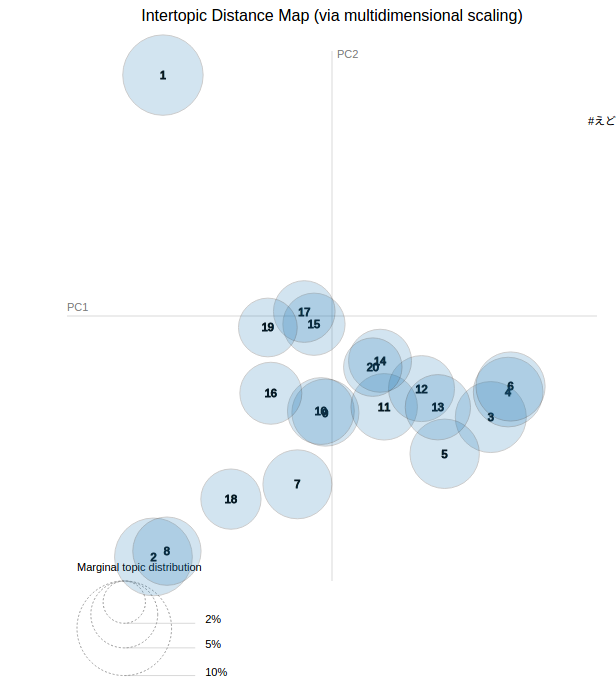
\includegraphics[width=\linewidth]{lda_vis_sep}
    \caption{Traditional LDA (tweets separated)}\label{fig:res_lda_vis_sep}
    \end{subfigure}
    \begin{subfigure}{.49\linewidth}
    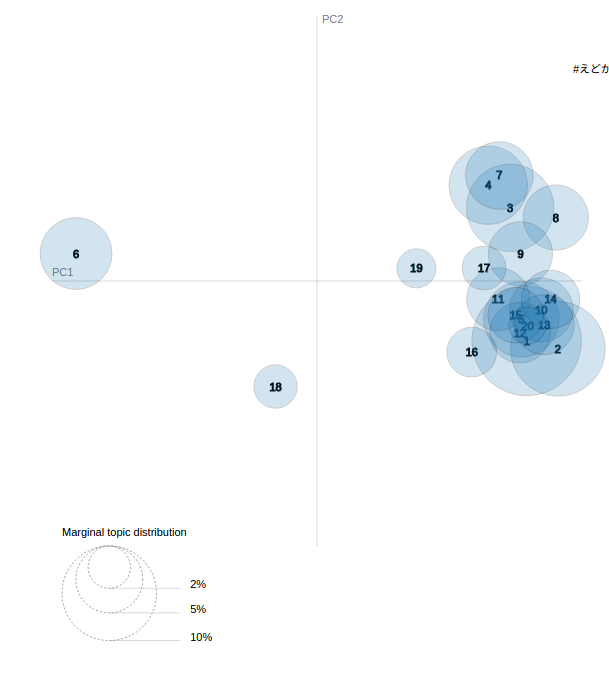
\includegraphics[width=\linewidth]{lda_vis_grp}
    \caption{Author-topic LDA (tweets aggregated)}\label{fig:res_lda_vis_grp}
    \end{subfigure}
    
    \caption{Traditional LDA \& author-topic model topic distribution visualised by LDAVis.}
    \label{fig:res_trad_var}
\end{figure}

\subsection{Topic description: a word topic example}

Let us take one example of the word topics shown in all the experiments to show how each method treated the corpus. The word topics 'shoes' (7 times) and 'size' (11 times) are among the most frequent words (they appear in at least one topic in every method).  

In the traditional LDA (with tweets separated), both words appear only in one topic (Topic 11), with words like `air', `jordan' and `nike', framing a very clear topic, the very popular sneakers in the 1980's and 90's (July is the release month every year for the retro-ed versions). This is also what happens in the Doc2Vec method with the tweets separated.  

On the other hand, in the LDA using author-topic, the word topic `size' appears five times, in two topics (Topic 10 and 11), and both of them seem to talk about the same shoes, but the other three (Topics 3, 4 and 19) do not have any specific topic, as shown by the judge agreement topic and meaningfulness agreement. The same happens with the Doc2Vec using the author-topic method. The word 'size' appears in three topics (Topics 6, 11 and 18), with one of them not attached to any specific topic, as shown by the same judgement scores.

This also would support our intuitions, namely, the tweets-separated methods provide better results than the author-topic ones, and Doc2vec provides more fine-grained results than LDA. 

\section{Influencers mining}

After having topics mined from our data, we attempted to implement a topic-sensitive influencers mining approach by combining PageRank and document-topic distribution.

\subsection{PageRank}
Page Rank was the first link analysis algorithm used by Google Search to rank websites in their search engine results, by assigning a numerical weighting to each element of a hyperlinked set of documents. The underlying assumption is that the most important websites are more likely to receive more links from other websites, therefore, it counts the number and quality of links to estimate how important a website is.
% TODO: Write more about PageRank in concept

\subsection{Topic-sensitive PageRank}
Weng et al. (2010) used  TwitterRank and showed it outperforms other algorithms used to measure micro-blogging sites, including the original PageRank and the one used by Haveliwala (2002) \cite{haveliwala_2002}. TwitterRank basically measures influence taking both the topical similarity between users and the link structure into account.
% TODO: present topic-sensitive PageRank

In Figure \ref{fig:topic_2_pagerank}, $\sum_{t=1}^{T}{DT_{d,t}} = 1, \forall 1\le d\le D$.

\begin{figure}[H]
	\centering
	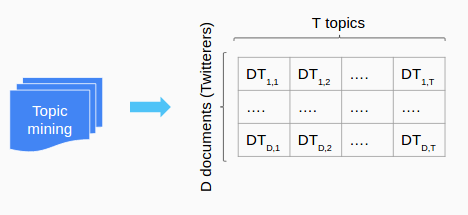
\includegraphics[scale=0.7]{topic_2_pagerank}
	\caption{Output from topic mining needed for PageRank.}
	\label{fig:topic_2_pagerank}
\end{figure}

With the topic-user distribution matrix above, we then perform the PageRank algorithm with a slight modification. On each edge from node $i$ to node $j$ in the graph, we assign a weight of
\[P_t(i,j)=\frac{T_j}{\sum{a:s_i\to s_a|T_a|}}*sim_t(i,j)\]
where $sim_t(i,j)=1-|DT_{i,t}-DT_{j,t}|$.

\subsection{Difficulties \& future improvements}

While implementing our approach, we found some challenging obstacles. Firstly, the Twitter REST API only allows us to query 15 user ids per a window of 15 minutes. Our proposed solution was to make queries in a priority queue, where users with the most tweeted tweets were queried first. With this approach, we successfully obtained the followers of the top 1,600 users. Nevertheless, the second problem appeared at this stage, which can be described as follows:


\begin{listing}[H]
    \begin{minted}{python}
df_users = pd.read_pickle('./data/data_user_selected_full.pkl')
t1 = df_users.apply(lambda row: len(row['inner_group']), axis = 1)
t1.describe()
    count    1600.0
    mean        0.0
    std         0.0
    min         0.0
    25%         0.0
    50%         0.0
    75%         0.0
    max         0.0
    dtype: float64
t2 = df_users.apply(lambda row: len(row['outer_group']), axis = 1)
t2.describe()
    count    1.600000e+03
    mean     1.833375e+04
    std      5.810536e+04
    min      1.000000e+00
    25%      4.405000e+02
    50%      3.314000e+03
    75%      1.895000e+04
    max      1.398493e+06
    dtype: float64
    \end{minted}
\end{listing}

In the code snippet above, the number of followers for each users (outer\_group) range from 1 to $1.4\times 10^6$ with an average of $2\times 10^4$. On the other hand, the number of followers that are in the group of 1,600 (inner\_group) is always zero. This lead to the failure of PageRank, as by no followers in the inner group, our graph will just be divided into 1,600 strong-connected components. With these 1,600 strong-connected components for each user, our 1,600 users have no influence on the others.

To overcome this problem, another data acquiring method should be performed instead. We suggest implementing the breadth-first search (BFS) algorithm to re-connect our separated strong-connected components with the 1,600 users as starting vertexes. Then, our BFS algorithm expands the graph by tracing the followers of each starting user follower. This iteration continues until we significantly reduce the number of connected components, it is expected to be performed in finite steps, backed up by the finite degrees of separation in social networks (3.5 from a report using Facebook\footnote{https://research.fb.com/three-and-a-half-degrees-of-separation/}).

\section{Conclusion}
The results from the experiments show that our proposed method with Doc2Vec and clustering method (K-means) outperforms the traditional LDA and its variant of author-topic model in topic mining for random tweets in Twitter. Not only with the meaningfulness from discovered topics, our proposed method also removed the need of unnecessary assumptions on the data.

We also found that the author-topic LDA did not perform as well as the traditional LDA. That confirms our doubts about the assumption made by the author-topic method to make LDA work in short-text documents, especially on micro-blogging sites.

On the other hand, our attempt to re-implement the TwitterRank methods failed due to obstacles from the data. To solve this, we suggest an alternative data acquisition by breadth-first search on the graph of our data-ready users.

\bibliographystyle{IEEEtran}
\bibliography{report}

\begin{appendices}

\section{Topic mining raw results with LDA}

\begin{table}
    \centering
    \begin{tabular}{|p{\linewidth}|}
    \hline
    Topic 0: 05 lady gaga link check \#mtvstars days utc \#mtvhottest bio spotted boom best stock convention united click win yet double\\
    Topic 1: game job art apply believe alert photo guy baby watch caught beat home return hits meet gets went amazing loves\\
    Topic 2: back want people tweet new video great twitter like see ever feel boys day full town get done via another\\
    Topic 3: 09 22 18 ut going \#ascendant listen 08 luck ac looking keep \#mediumcoeli mc download different 07 \#ipl 4 high\\
    Topic 4: new \#deals black end iphone apple case date buy app post 2 caps games \#iphone cover mini bag 4 6\\
    Topic 5: trump clinton get hillary special donald free email list tips access join \#home vote updates frog f bet resolved priority\\
    Topic 6: 31 shirt sz time \#gamedev new started late second \#final 5 boost \#indiedev yeezy shocking destination 2 f reached cool\\
    Topic 7: 2016 july pm \#U+3048 U+3069 U+304C U+308F U+30A4 U+30B1 U+30E1 U+30F3 tos null mdbjss xxx 11 ca afe 20 s0t 12345 gun trends trending 7 gundam cat\\
    Topic 8: go got year playing let thing high friends 19 one ever would mom life like 27 every smile enough pokemon\\
    Topic 9: code 10 use get like 15 20 25 free available sale wear order https shipping gold lit summer would shop\\
    Topic 10: 3ndback \#jobs media via social marketing business service read turn morning internet taking \#business new customer xbox \#marketing sales line\\
    Topic 11: black size new nike white air top 12 shoes \#shoes blue jordan season 1 mens dress red men episode 10\\
    Topic 12: beautiful girl see 23 heart 29 home away part mind following 01 woman flight man boss name things speech feet\\
    Topic 13: may latest design inc \#tech new course hey piping body price make institute want perfect food \#news check \#amazon signs\\
    Topic 14: love follow u work please today get happy c thank always much world wanted never experience ur someone best hi\\
    Topic 15: 21 26 via 04 r w card page america offer degree college fire top future amazon spend important 10 credit\\
    Topic 16: 30 need things know girls right life give people really like guys get play fuck wrong never remember still talk\\
    Topic 17: one three try million hundred ah sign free two west could killed follow update thousand exit give us new five\\
    Topic 18: look good photos must police stop music \#urbanattires \#euro2016 years 100 see found shop sex later place worth site like\\
    Topic 19: 06 crzx\_omg \#news join us says president dead nice police news attack one report france obama son streaming paul rio\\
    \hline
    \end{tabular}
	\caption{LDA (tweets separated) raw result}
	\label{tb:res_lda_sep_raw}
\end{table}

\begin{table}[H]
	\centering
	\begin{tabular}{| l | l | r | l | r | r | r | r | r |}
		\hline
		& \multicolumn{2}{c|}{\textbf{1st judge}} & \multicolumn{2}{c|}{\textbf{2nd judge}} & \multicolumn{2}{c|}{\textbf{Agreement}} & \multicolumn{2}{c|}{\textbf{Average}}\\
        \cline{2-9}
         & \textbf{Topic} & \textbf{Score} & \textbf{Topic} & \textbf{Score} & \textbf{1st} & \textbf{2nd} & \textbf{Score} & \textbf{Agree.}\\
		\hline
            0 & mtv event & 6 & mtv & 5 & 10 & 10 & 5.5 & 10\\
            1 & pics & 5 & NA & 0 & 8 & 7 & 2.5 & 7.5\\
            2 & people \& video & 0 & NA & 0 & 10 & 10 & 0 & 10\\
            3 & music \& numbers & 2 & NA & 0 & 10 & 8 & 1 & 9\\
            4 & phones & 6 & tech gadget & 8 & 9 & 9 & 7 & 9\\
            5 & us elections scandals & 7 & US election & 7 & 10 & 10 & 7 & 10\\
            6 & gaming & 4 & NA & 0 & 8 & 7 & 2 & 7.5\\
            7 & numbers & 0 & NA & 0 & 10 & 10 & 0 & 10\\
            8 & pokemon go & 3 & NA & 0 & 9 & 8 & 1.5 & 8.5\\
            9 & sales ads & 6 & online sales & 4 & 10 & 9 & 5 & 9.5\\
            10 & business & 4 & tech company & 7 & 7 & 8 & 5.5 & 7.5\\
            11 & shoes & 5 & shoes & 5 & 10 & 10 & 5 & 10\\
            12 & talk on ads & 0 & feelings & 1 & 9 & 6 & 0.5 & 7.5\\
            13 & sales & 0 & tech company & 4 & 8 & 6 & 2 & 7\\
            14 & motivational & 4 & feelings & 5 & 10 & 5 & 4.5 & 7.5\\
            15 & college & 3 & NA & 0 & 9 & 6 & 1.5 & 7.5\\
            16 & woman magazine & 7 & NA & 0 & 5 & 3 & 3.5 & 4\\
            17 & numbers \& news & 0 & NA & 0 & 10 & 2 & 0 & 6\\
            18 & news \& sales & 0 & NA & 0 & 10 & 5 & 0 & 7.5\\
            19 & news & 6 & politics & 7 & 9 & 6 & 6.5 & 7.5\\
		\hline
	\end{tabular}
	\caption{Scoring for LDA (tweets separated)}
	\label{tb:res_lda_sep}
\end{table}

\begin{table}
    \centering
    \begin{tabular}{|p{\linewidth}|}
    \hline
    Topic 0: code shop pinned tweet available wear sale https order \#tech another share lit gold \#fashion \#apple sex \#urbanattires check incident\\
    Topic 1: currently mind heart pm thank double following \#nowplaying fairy quote \#jobs code johnson part \#nfl someone handbag hi dark \#soulecting\\
    Topic 2: resolved join play \#pushawardslizquens gbp streaming invite part code page 01 bet someone https \#bigdata bid news bonus business pm\\
    Topic 3: \#news photos via ut size sex nike null jordan air \#mediumcoeli post source tumblr \#ascendant house sign plz ac give\\
    Topic 4: via boys news town ebay vintage r deal size bid \#adult share w https set published apple \#sex blue escorts\\
    Topic 5: buy pm beautiful mind following \#U+3048 U+3069 U+304C U+308F U+30A4 U+30B1 U+30E1 U+30F3 vol \#deals direction nothing places others blessed humble fashion \#ebay via \#growthhacking \#special \#cheap\\
    Topic 6: lady gaga check days offer stock \#health win apply personalized via deals \#deals business \#home found \#jobs human xxx \#hr\\
    Topic 7: pm tos \#U+3048 U+3069 U+304C U+308F U+30A4 U+30B1 U+30E1 U+30F3 null afe 11 16 17 14 26 21 29 13 18 25 08 09 22 24 07\\
    Topic 8: \#U+3048 U+3069 U+304C U+308F U+30A4 U+30B1 U+30E1 U+30F3 pm tos mdbjss follow \#gamedev ca tweet \#indiedev 25 app 16 win gbp 24 gun 1l 27 29 post\\
    Topic 9: course \#mtvhottest follow gaga lady design institute \#jobs \#mgwv trump engineering via certified qa qc retweet gain code police \#followtrick\\
    Topic 10: \#shoes nike size air shoes price \#news low jordan ah listen null 11 jul retro mens far red gold pm\\
    Topic 11: size air shoes \#deals nike jordan baby \#amazon mens sz listen red someone 90s 80s blue 24hrs hiphop 11 9\\
    Topic 12: utc spotted may check latest \_ hey updates inc bid \#nowplaying camera follow via jul event photos associated notification please\\
    Topic 13: pm s0t xxx tweet hi hope happy code \#football thanks \#steelers steelers \#pittsburgh via meet poncho \#cricket customer pizza holy\\
    Topic 14: following code please c mm temperature rain mind barometer hpa null wind dream smile follow humidity trump business pm started\\
    Topic 15: null code episode season offer card w join list special updates access spend terms email receive connected f credit pm\\
    Topic 16: \#news code silver sale \#silver f page buy pm temp floor follow available dollar 3rd \#mgwv amazon flight set product\\
    Topic 17: jobs \#home hello experience trending follow graduate wanted tips \#news decor check improvement trends \#gardening read pm sorry daily code\\
    Topic 18: \#jobs jul beds scheduled baths \#ipl bus remark thank following gate someone mind due mins lego everything person woman \#build\\
    Topic 19: shirt code hundred \#euro2016 luck give try \#final app three hi ah million classroom size \#news thousand \#tech buy h\\
    \hline
    \end{tabular}
	\caption{LDA (author-topic) raw result}
	\label{tb:res_lda_grp_raw}
\end{table}

\begin{table}[H]
	\centering
	\begin{tabular}{| l | l | r | l | r | r | r | r | r |}
		\hline
		& \multicolumn{2}{c|}{\textbf{1st judge}} & \multicolumn{2}{c|}{\textbf{2nd judge}} & \multicolumn{2}{c|}{\textbf{Agreement}} & \multicolumn{2}{c|}{\textbf{Average}}\\
        \cline{2-9}
         & \textbf{Topic} & \textbf{Score} & \textbf{Topic} & \textbf{Score} & \textbf{1st} & \textbf{2nd} & \textbf{Score} & \textbf{Agree.}\\
		\hline
            0 & sales & 5 & online shopping & 1 & 8 & 6 & 3 & 7\\
            1 & magazine \& sports & 0 & NA & 0 & 10 & 7 & 0 & 8.5\\
            2 & betting & 0 & NA & 0 & 10 & 7 & 0 & 8.5\\
            3 & shoes \& sex & 0 & NA & 0 & 10 & 9 & 0 & 9.5\\
            4 & toys in ebay & 2 & NA & 0 & 10 & 8 & 1 & 9\\
            5 & offers & 2 & online sales & 2 & 10 & 9 & 2 & 9.5\\
            6 & offers & 1 & NA & 0 & 10 & 4 & 0.5 & 7\\
            7 & numbers & 0 & NA & 0 & 10 & 8 & 0 & 9\\
            8 & gaming \& numbers & 0 & NA & 0 & 10 & 7 & 0 & 8.5\\
            9 & tutti-frutti news & 0 & mtv & 1 & 10 & 3 & 0.5 & 6.5\\
            10 & shoes & 1 & shoes & 2 & 10 & 9 & 1.5 & 9.5\\
            11 & shoes \& music & 0 & shoes & 2 & 10 & 7 & 1 & 8.5\\
            12 & news agency & 1 & NA & 0 & 10 & 2 & 0.5 & 6\\
            13 & football & 6 & NA & 0 & 7 & 2 & 3 & 4.5\\
            14 & forecast & 5 & weather & 4 & 10 & 9 & 4.5 & 9.5\\
            15 & offers & 3 & NA & 0 & 9 & 4 & 1.5 & 6.5\\
            16 & stock market news & 5 & NA & 0 & 8 & 2 & 2.5 & 5\\
            17 & housing & 4 & NA & 0 & 8 & 0 & 2 & 4\\
            18 & lego? & 0 & NA & 0 & 10 & 0 & 0 & 5\\
            19 & sports ads & 4 & NA & 0 & 9 & 2 & 2 & 5.5\\
		\hline
	\end{tabular}
	\caption{Scoring for LDA (author-topic)}
	\label{tb:res_lda_grp}
\end{table}

\section{Topic mining raw results with Doc2Vec \& K-means}

\begin{table}[H]
    \centering
    \begin{tabular}{|p{\linewidth}|}
    \hline
    Topic 0: follow free join updates euro2016 tweet luck good shirt offer win want work email final check bio hello card matriculant\\
    Topic 1: july 2016 pm U+3048 U+3069 U+304C U+308F U+30A4 U+30B1 U+30E1 U+30F3 tos null mdbjss xxx afe 01 29 17 08 09 ca 26 24 12 05 21\\
    Topic 2: trump clinton hillary donald convention bernie dnc obama sanders vote speech president news republican gop campaign democratic says america election\\
    Topic 3: gaga lady mtvhottest just love resolved huuugs post new need want mtvstars utc cest beautiful home 3ndback tweet like salute\\
    Topic 4: marketing tech business news content howto social internet new media socialmedia growthhacking app gamedev google seo smm online tips indiedev\\
    Topic 5: photos woman girl wife years later mom sex girlfriend daughter man photo dad looks guy shocking video gets caught pregnant\\
    Topic 6: shoes size nike air jordan black retro mens sz white new adidas 11 running sneakers red grey 12 10 blue\\
    Topic 7: police news attack turkey killed says man shooting dallas dead china coup death new state south officers nice shot isis\\
    Topic 8: code use like shop available 15 wear 10 lit urbanattires order sale shipping https dope caps discount free gold promo\\
    Topic 9: vintage silver ebay fashion set jewelry necklace home gold antique handmade art new bid decor bracelet bag gift bestservice exotic\\
    Topic 10: sex things know life people make way women best time better ways girls health men need guys signs just degree\\
    Topic 11: iphone apple new black bid ipad app smartphone 16gb games deals unlocked samsung galaxy case xbox wireless free mac ebay\\
    Topic 12: spotted ut 2016 utc wind jul humidity ascendant mins rain mediumcoeli today reached destination hpa mc temp started ac temperature\\
    Topic 13: love mind following heart beautiful people thank person know happy just make life like dear follow best thing things want\\
    Topic 14: like just got shit fuck playing love wanna high girl know people ur sides want switchy score bae need think\\
    Topic 15: football nfl nba browns steelers cleveland pittsburgh card jersey tickets basketball topps deals boston new cards wwe ebay mlb celtics\\
    Topic 16: black dress sleeve size handbag new nwt leather purse pink bag blue neck tunic poncho fashion shirt sleeveless white betsey\\
    Topic 17: job jobs apply alert opportunity manager piping course sales career corp company business group new aptask hiring assistant institute investment\\
    Topic 18: ah million thousand win news vs hamilton soccer open 2016 new england cricket final australian tour manchester team united lady\\
    Topic 19: episode season nowplaying new download listen free music book watch rock popcorntime offline fullblastradio books star love unabridged thepiratebay hiphop\\
    \hline
    \end{tabular}
	\caption{Doc2Vec \& K-means (tweets separated) raw result}
	\label{tb:res_doc_sep_raw}
\end{table}

\begin{table}[H]
	\centering
	\begin{tabular}{| l | p{2.7cm} | r | p{2.7cm} | r | r | r | r | r |}
		\hline
		& \multicolumn{2}{c|}{\textbf{1st judge}} & \multicolumn{2}{c|}{\textbf{2nd judge}} & \multicolumn{2}{c|}{\textbf{Agreement}} & \multicolumn{2}{c|}{\textbf{Average}}\\
        \cline{2-9}
         & \textbf{Topic} & \textbf{Score} & \textbf{Topic} & \textbf{Score} & \textbf{1st} & \textbf{2nd} & \textbf{Score} & \textbf{Agree.}\\
		\hline
            0 & euro2016 ads & 6 & NA & 0 & 7 & 3 & 3 & 5\\
            1 & numbers & 0 & NA & 0 & 10 & 10 & 0 & 10\\
            2 & us election & 10 & US election & 10 & 10 & 10 & 10 & 10\\
            3 & mtv event \& lady gaga & 7 & mtv & 4 & 9 & 9 & 5.5 & 9\\
            4 & marketing, tech \& media & 8 & entrepreneur \& startup & 10 & 8 & 7 & 9 & 7.5\\
            5 & a news scandal & 7 & family & 3 & 6 & 6 & 5 & 6\\
            6 & sport shoes & 8 & shoes & 10 & 10 & 10 & 9 & 10\\
            7 & international news & 6 & world news & 9 & 9 & 10 & 7.5 & 9.5\\
            8 & shopping & 7 & online sale & 8 & 10 & 7 & 7.5 & 8.5\\
            9 & expensive shopping & 9 & jewelry & 7 & 10 & 8 & 8 & 9\\
            10 & magazine articles on sexual life & 8 & NA & 0 & 5 & 5 & 4 & 5\\
            11 & phones & 10 & tech gadget & 9 & 10 & 8 & 9.5 & 9\\
            12 & forecast & 8 & weather & 4 & 9 & 9 & 6 & 9\\
            13 & love & 8 & feelings & 5 & 9 & 7 & 6.5 & 8\\
            14 & tennagers stuff & 4 & life & 1 & 7 & 5 & 2.5 & 6\\
            15 & us sports & 10 & sports & 7 & 9 & 8 & 8.5 & 8.5\\
            16 & womens clothes & 9 & fashion & 8 & 10 & 9 & 8.5 & 9.5\\
            17 & job & 8 & business & 7 & 9 & 6 & 7.5 & 7.5\\
            18 & other sports & 8 & sports & 5 & 9 & 7 & 6.5 & 8\\
            19 & download video \& music & 6 & multimedia & 7 & 10 & 8 & 6.5 & 9\\
		\hline
	\end{tabular}
	\caption{Scoring for Doc2Vec \& K-means (tweets separated)}
	\label{tb:res_doc_sep}
\end{table}

\begin{table}
    \centering
    \begin{tabular}{|p{\linewidth}|}
    \hline
    Topic 0: code use like shop available lit wear 15 urbanattires https 10 order shipping sale discount dope caps free promo checkout\\
    Topic 1: gbp mtvhottest follow gaga utc tweet free hi mgwv lady post spotted classroom following resolved humidity hpa love followtrick mtvstars\\
    Topic 2: jobs corp rating zacks communityscene plc assistant published investment hiring job llc research shares manager news earnings management engineer opportunity\\
    Topic 3: people sex things girls shocking girl mom porn just make know like woman photos life daughter happens confessions pictures later\\
    Topic 4: radiohead prince app unabridged hamilton iphone whatsapp ipad mac tvseries paulmccartney utilities rend games metgala drama 2016 nonfiction new comedy\\
    Topic 5: like want need love just life people ur girl got know shit beautiful time drake bae bio wanna make look\\
    Topic 6: bid size shoes black nike new apple mens 16gb air leather sz jordan white unlocked iphone retro deals silver ebay\\
    Topic 7: sex later woman wife girl years photos dad like mom doctors happens girlfriend shocking unthinkable guy looks just looked girls\\
    Topic 8: news trump police clinton new says hillary attack donald china reuters convention brexit obama business people killed turkey ap dallas\\
    Topic 9: photos apply alert sex job nigeria nigerian buhari position video lagos photo pics limited manager penis things officer ways porn\\
    Topic 10: pushawardslizquens twain love shakespeare law people mark like life just good time things make man know william aldubiyamin8days person think\\
    Topic 11: vintage sleeve fashion nfl black jewelry size silver leather new handbag dress nba football handmade tunic dvd necklace purse nwt\\
    Topic 12: new trump police says clinton brexit 39 2016 watch man update attack news convention france dallas rio hillary china donald\\
    Topic 13: hillary trump clinton bernie neverhillary dnc https vote sanders demexit berniesanders bernieorbust demsinphilly feelthebern people hrc just obama 4bernie america\\
    Topic 14: nonsense friendliness hickman statutes acronym goblin manipulative titan flee floating unfunny triton groundswell maximal unicycle tubeless peaked shotgunning persia shortens\\
    Topic 15: july 2016 U+3048 U+3069 U+304C U+308F U+30A4 U+30B1 U+30E1 U+30F3 pm tos null mdbjss afe xxx s0t 01 ca 09 08 ut 07 02 ascendant 05 06\\
    Topic 16: like love just people want life need ur person know things really feel isolated girl vocals make signs shit feelings\\
    Topic 17: https follow win nowplaying new love like just good gamedev thank thanks today happy asmsg giveaway hi free day book\\
    Topic 18: men size sunglasses company filing profile new llc sec sale nwt tie ashtray collectible women porcelain neck silk ralph listing\\
    Topic 19: marketing business health tech socialmedia seo deals growthhacking startup contentmarketing content smm startups bitcoin howto bigdata entrepreneur blockchain realtor social\\
    \hline
    \end{tabular}
	\caption{Doc2Vec \& K-means (author-topic) raw result}
	\label{tb:res_doc_grp_raw}
\end{table}

\begin{table}[H]
	\centering
	\begin{tabular}{| l | p{2.7cm} | r | p{2.7cm} | r | r | r | r | r |}
		\hline
		& \multicolumn{2}{c|}{\textbf{1st judge}} & \multicolumn{2}{c|}{\textbf{2nd judge}} & \multicolumn{2}{c|}{\textbf{Agreement}} & \multicolumn{2}{c|}{\textbf{Average}}\\
        \cline{2-9}
         & \textbf{Topic} & \textbf{Score} & \textbf{Topic} & \textbf{Score} & \textbf{1st} & \textbf{2nd} & \textbf{Score} & \textbf{Agree.}\\
		\hline
        0 & shopping & 6 & online shopping & 7 & 10 & 9 & 6.5 & 9.5\\
        1 & mtv event & 6 & mtv & 5 & 10 & 10 & 5.5 & 10\\
        2 & jobs & 2 & business & 7 & 6 & 5 & 4.5 & 5.5\\
        3 & sexual scandal & 4 & sex \& life & 2 & 9 & 8 & 3 & 8.5\\
        4 & music \& tech & 6 & multimedia & 7 & 9 & 7 & 6.5 & 8\\
        5 & love music & 7 & feelings & 5 & 8 & 6 & 6 & 7\\
        6 & shoes \& phones & 0 & online shopping & 7 & 4 & 6 & 3.5 & 5\\
        7 & news scandal & 7 & family & 2 & 6 & 3 & 4.5 & 4.5\\
        8 & politics news & 6 & politics & 9 & 9 & 9 & 7.5 & 9\\
        9 & african dontknowwhat & 0 & porn & 6 & 6 & 7 & 3 & 6.5\\
        10 & writers & 3 & literature & 4 & 10 & 9 & 3.5 & 9.5\\
        11 & expensive shopping & 8 & fashion & 9 & 9 & 8 & 8.5 & 8.5\\
        12 & mainly us news & 6 & world news & 6 & 9 & 7 & 6 & 8\\
        13 & us elections & 8 & US election & 10 & 10 & 10 & 9 & 10\\
        14 & fancy writing style & 0 & NA & 0 & 10 & 7 & 0 & 8.5\\
        15 & numbers & 0 & NA & 0 & 10 & 10 & 0 & 10\\
        16 & women magazine talk & 8 & feelings & 5 & 7 & 4 & 6.5 & 5.5\\
        17 & ads & 5 & NA & 0 & 8 & 4 & 2.5 & 6\\
        18 & shopping items & 7 & sale & 4 & 9 & 6 & 5.5 & 7.5\\
        19 & marketing & 8 & tech entrepreneur \& startup & 10 & 8 & 7 & 9 & 7.5\\
		\hline
	\end{tabular}
	\caption{Scoring for Doc2Vec \& K-means (author-topic)}
	\label{tb:res_doc_grp}
\end{table}

\end{appendices}


\end{document}
